% =========================================================================
% main.tex --- draft v1 (cycle 6)
% Target: Structural and Multidisciplinary Optimization (regular paper).
% Drafted in plain article class for portability; convert to the Springer
% Nature template (sn-jnl.cls, spbasic bibliography) at submission time.
%
% Sources: notes/paper_skeleton.md (+ patch v2 in notes/review_gpt_response.md
% section 4, + patch v3 in notes/cycle5_note.md section 6). Claim diet:
% paper_skeleton.md section 6. All numbers traceable to notes/cycle1..5.
%
% TODO before submission:
%   [ ] author list, affiliations, ORCID, funding, data-availability URL
%   [x] bibliography verified 2026-08-16 (ananiev2005 DOI, li2020fixedpoint
%       replaces the MS thesis, kim2025simpl = published SMO 68 version,
%       groenwold2009gss added; Munro reference resolved as nonexistent ---
%       see comment in refs.bib). Residual: spot-check page numbers of the
%       classical entries against publisher records.
%   [~] publication figures (backlog 3): fig_cycle5 split DONE
%       (fig_psweep_pub.png, fig_negbranch.png via src/c5_fig_pub.py);
%       remaining: redraw Fig 1 toy schematic, restyle Figs 2-5 to match
%   [ ] Springer template conversion + spbasic style
% =========================================================================
\documentclass[11pt,a4paper]{article}
\usepackage[margin=2.7cm]{geometry}
\usepackage{amsmath,amssymb,amsthm}
\usepackage{graphicx}
\usepackage{booktabs}
\usepackage{natbib}
\usepackage[colorlinks=true,linkcolor=blue,citecolor=blue,urlcolor=blue]{hyperref}
\graphicspath{{../figs/}}

\newtheorem{proposition}{Proposition}
\newtheorem{remark}{Remark}
\newcommand{\smax}{s_{\max}}
\newcommand{\smin}{s_{\min}}
\newcommand{\etastar}{\eta^{\star}}
\newcommand{\Dfilt}{\tilde{D}}
\newcommand{\todo}[1]{\textbf{[TODO: #1]}}

\title{Spectral dynamics of the damped optimality-criteria iteration:\\
flip and winner-take-all branches, thresholds,\\
and the marginality of $\eta=\tfrac12$}
\author{\todo{author list and affiliations}}
\date{Draft v1 --- August 16, 2026}

\begin{document}
\maketitle

% -------------------------------------------------------------------------
\begin{abstract}
The optimality-criteria (OC) update with numerical damping $\eta$ is the
workhorse of density-based topology optimization, yet the choice
$\eta=\tfrac12$ has remained folklore. Viewed as a dynamical system in
logarithmic coordinates, the damped OC map has local multipliers obeying
$\mu = 1-\eta s$ on the volume-constraint tangent space, with $s$ the
log--log stiffness of the filtered sensitivity field. Exact two-bar models
give both signs of $s$: a series model yields $s=p{+}1$, placing the
standard pair $(3,\tfrac12)$ exactly on the period-doubling boundary
$\etastar=2/s$ of the positive branch; a parallel model yields
$s=-(p{-}1)$, a winner-take-all instability. On an instrumented 88-line
benchmark, exactly projected finite-difference Jacobians confirm the law
at the operator level: $\eta$-invariant spectra, eigenmodes matching the
observed oscillation patterns, and rates matching $|1-\eta\,\smax|$ to
three decimals (42 mode-aligned probes, median deviation $0.001$). Across
$p\in[1.5,5]$, $\smax$ saturates at $p{+}1$ under a low-damping reference
protocol, while standard damping drifts to alternative fixed points with
$\smax\le 2/\eta$; the protocols separate exactly at $p=3$, and each fixed
point obeys its own threshold $2/\smax$. Moreover, since every measured
spectrum has its lower edge near $s=0$, the min--max optimal (Richardson)
damping coincides with the flip boundary to $1$--$2\%$: at $p=3$ the
folklore choice is not merely marginal but optimal, and lowering $\eta$
buys stability at the top of the spectrum at the documented cost of
slowing the bulk. We identify the negative branch
in the wild as benign symmetry breaking, and show that filtering detunes
the flip branch: larger sensitivity-filter radii lower $\smax$, and
density filtering pushes the threshold to $\etastar\approx5.4$, far
outside the practical range. Combined with the equivalence of
$\eta=\tfrac12$ to reciprocal intervening variables
\citep{groenwold2008}, the folklore damping is the approximation whose
curvature is exactly half the true curvature at $p=3$: the statics and the
dynamics of the OC method meet at the same constant.
\end{abstract}

% =========================================================================
\section{Introduction}\label{sec:intro}

Density-based topology optimization owes much of its practical success to an
update rule of striking simplicity. In the SIMP framework
\citep{bendsoe1989}, the optimality-criteria (OC) iteration rescales each
element density by a power of the ratio between its strain-energy sensitivity
and a volume multiplier,
\begin{equation}
  x_e^{+} \;=\; \mathrm{clip}\!\left( x_e B_e^{\eta} \right),
  \qquad
  B_e \;=\; \frac{-\partial c/\partial x_e}{\lambda\,\partial V/\partial x_e},
  \label{eq:oc}
\end{equation}
with a damping exponent $\eta$ and move limits; the multiplier $\lambda$ is
found by bisection so that the volume constraint holds. The educational
codes that shaped the field \citep{sigmund2001top99,andreassen2011top88}
hard-wire $\eta=\tfrac12$, and commercial implementations codify the same
folklore---smaller exponents are described as more stable but slower
\citep{abaqus_stressratio}---without a quantitative theory of what $\eta$
controls, why $\tfrac12$ works, or when it fails by oscillation.

This paper supplies that theory at the level where the phenomenon lives: the
iteration itself, viewed as a discrete dynamical system. Our starting point
is elementary. In logarithmic coordinates $z_e=\ln x_e$ the pure OC update
is an exponentiated-gradient-type multiplicative step, and its linearization
about a fixed point has, on the tangent space of the volume constraint, the
affine multiplier law
\begin{equation}
  \mu_m \;=\; 1-\eta\, s_m ,
  \label{eq:law}
\end{equation}
where $s_m$ are the eigenvalues of the (projected) negative log--log
sensitivity operator $\mathcal S = -P\,\partial \ln \Dfilt / \partial \ln x$.
Every question about damping becomes a question about the spectrum
$\{s_m\}$: modes with $s_m>0$ are stable for $\eta<2/s_m$ (flip boundary at
equality, one-step deadbeat at $\eta=1/s_m$), and modes with $s_m<0$ grow
monotonically for every $\eta>0$. Exact two-bar models anchor the two signs:
a series, statically determinate model has $s=p{+}1$ exactly, so the
standard pair $(3,\tfrac12)$ lies \emph{exactly on the flip boundary}; a
parallel model has $s=-(p{-}1)$, a winner-take-all competition. What
remained genuinely open---and occupies most of this paper---is whether these
constants survive contact with a real code, where the update composes a
finite-element solve, a sensitivity or density filter, a $\lambda$
bisection, clipping, and move limits.

They survive, and they do so at the operator level, not merely as trends.
Our contributions:

\begin{enumerate}
\item \textbf{Multiplier law and exact models.} The log-coordinate law
  \eqref{eq:law} with the stability window $\eta\in(0,2/s)$ of the positive
  branch, one-step damping $\eta=1/s$, and flip boundary $\etastar=2/s$;
  series and parallel two-bar models realizing $s=p{+}1$ and $s=-(p{-}1)$
  exactly (machine precision in the toys; bifurcation observed at
  $\eta=0.500$).
\item \textbf{Marginality of the standard recipe.} On the canonical
  $60\times20$ MBB benchmark with sensitivity filtering, the measured
  spectrum saturates at $\smax=3.974\approx p{+}1$, hence
  $\etastar=0.503$: the folklore damping $\eta=\tfrac12$ operates with a
  margin of $0.003$. Across meshes and boundary conditions the threshold
  stays within $13\%$ of the standard damping ($\smax\in[2.9,4.0]$ for
  sensitivity filtering at $p=3$), widening to $28\%$ at volume fraction
  $0.4$.
\item \textbf{An operator-level measurement program.} Exactly projected
  finite-difference Jacobians of the full update (volume tangent basis $Q$,
  row-null residual $\sim2\times10^{-4}$, and a constraint artifact at
  $s=1/\eta$ that the projection removes); $\eta$-invariant $s$-spectra
  (three decimals); the trajectory identity $\hat\mu=1-\eta\hat s$ in 28
  unconstrained runs (three decimals); eigenmode--oscillation coincidence
  ($|\cos|\ge0.93$); and sub- and super-threshold rates matching
  $|1-\eta\smax|$ to three decimals.
\item \textbf{Saturation and dynamic self-limiting.} Under a low-damping
  reference protocol, $\smax$ saturates at $p{+}1$ across the whole sweep
  $p\in[1.5,5]$ (saturation ratio $0.96$--$0.995$). Runs converged at the
  standard damping instead drift to fixed points with $\smax\le2/\eta$;
  the two protocols separate exactly at $p{+}1=2/\eta$, i.e.\ $p=3$ for
  $\eta=\tfrac12$. Onset thresholds measured behaviorally follow each fixed
  point's own $2/\smax$---the threshold is a property of the fixed point
  the dynamics selects.
\item \textbf{The negative branch in the wild.} The parallel-model
  instability appears in real spectra as $\smin<0$: a symmetry-breaking
  redistribution among low-density mirror pairs that grows at the predicted
  rate $1-\eta\smin$ (four decimals) and terminates by resettling into a
  nearby asymmetric fixed point whose spectrum has shed the negative
  eigenvalue, at essentially unchanged compliance. Accordingly, $2/\smax$
  must be stated as the flip boundary \emph{of the positive branch}, not as
  a global stability window.
\item \textbf{Filtering as detuning, and practical guidance.} Enlarging the
  sensitivity-filter radius lowers $\smax$ (at $p=5$ from $5.97$ to $2.95$
  between $r_{\min}=1.1$ and $2.4$; mildly at $p=3$), and density filtering
  collapses it to $0.37$ ($\etastar\approx5.4$; no flip for $\eta\le4$
  across seeds; behavioral onset bracketed in $(5.4,6.0]$). The folk
  remedies for OC oscillation---reduce $\eta$, or switch to density
  filtering---are two faces of the same constant $2/\smax$.
\item \textbf{Statics--dynamics synthesis.} \citet{groenwold2008} proved
  that OC damping is equivalent to exponential intervening variables with
  $\eta=1/(1-a)$, and that $\eta=\tfrac12$ is exactly the reciprocal
  approximation. Our law gives that equivalence a dynamical meaning: at
  $p=3$ the reciprocal curvature is exactly half the true curvature, which
  is precisely the multiplier $\mu=-1$. The one-step damping $\eta=1/(p+1)$
  is, in their dictionary, the exact exponential fit $a=-p$---implicit in
  their framework, made explicit here as the midpoint of the stability
  window.
\end{enumerate}

Everything is measured on instrumented variants of the 88-line code
\citep{andreassen2011top88} with full reproduction scripts; no claim in
this paper rests on the toys alone.

% =========================================================================
\section{Related work}\label{sec:related}

\paragraph{Convergence of the problem formulation.} A classical line of
work addresses the SIMP \emph{problem}---existence, effect of the
penalization exponent, interpolation schemes---rather than the iteration:
\citet{rietz2001} on sufficiency of a finite exponent,
\citet{stolpe2001} on interpolation, and \citet{martinez2005} on
theoretical convergence properties of the method under weakened
assumptions. These results are orthogonal to ours: they concern what is
being solved, not the dynamics of the solver.

\paragraph{Resizing iterations as dynamical systems.} The closest
dynamical precedent is the fully-stressed-design (FSD) literature.
\citet{mueller2001} showed that some fully stressed frames are
\emph{unstable fixed points} of the stress-ratio iteration and therefore
unreachable by conventional resizing; follow-ups mapped multiple load
paths and multiplicity \citep{mueller2002,liu2003}, continuing a lineage
that goes back to \citet{razani1965} and includes engineering variants
such as MFUD \citep{patnaik1998mfud}. These works established the view
``resizing iteration = dynamical system, fixed points carry stability
labels''---for trusses and frames, at $\eta=1$, without damping as a
bifurcation parameter, without a multiplier law or flip threshold, and
without measured spectra. We import their viewpoint into density-based
topology optimization and make it quantitative. More recently,
\citet{li2020fixedpoint} treated the OC iteration explicitly as a
fixed-point map and accelerated it by Anderson extrapolation---the
oscillations they mitigate are the flip branch we analyze.

\paragraph{The statics of $\eta$.} What $\eta$ \emph{is}, in approximation
terms, is settled ground: \citet{groenwold2008} proved the equivalence of
damped OC to dual sequential approximate optimization with exponential
intervening variables, $\eta=1/(1-a)$, identifying $\eta=\tfrac12$ with the
reciprocal approximation ($a=-1$) and advocating adaptive exponents
\citep[see also][]{groenwold2007ise}; the same line engineered further
exponent-family variants of the update itself
\citep{groenwold2009gss}. Svanberg's CCSA established that
non-conservative separable approximations can cycle and that
conservatization restores convergence \citep{svanberg2002ccsa}, with MMA
the canonical practical realization \citep{svanberg1987mma}. None of these
works analyzes the damped OC map as a dynamical system or measures its
spectra; our results are the dynamical complement to their statics, and we
attribute the $\eta$--$a$ dictionary entirely to them.

\paragraph{Modern convergent algorithms.} \citet{ananiev2005} interpreted
the OC update as a projected gradient method; recent work builds provably
convergent mirror-descent schemes, notably SiMPL with Fermi--Dirac
entropy \citep{kim2025simpl,keith2024simpl}, whose authors describe
classical OC as a heuristic whose theoretical basis is still being
developed. Our contribution is complementary: we do not propose a new
algorithm, we supply the local theory---and the measurements---of the one
everybody already runs. Filtering, which will turn out to control the
spectrum, enters through the standard constructions
\citep{sigmund1998numerical,bourdin2001}.

% =========================================================================
\section{Theory}\label{sec:theory}

\subsection{The damped OC map in logarithmic coordinates}

Consider compliance minimization with a volume equality constraint and the
update \eqref{eq:oc}. Write $z_e=\ln x_e$ and let $\Dfilt_e$ denote the
filtered sensitivity entering the update. On the \emph{free set} $F$
(elements pinned neither by the box bounds nor by move limits) the pure OC
step reads
\begin{equation}
  z^{+} \;=\; z + \eta\left(\ln \Dfilt(z) - \ln\lambda(z)\,\mathbf 1\right),
  \label{eq:logstep}
\end{equation}
an exponentiated-gradient-type update in which the logarithm of the
sensitivity field plays the role of the gradient; this log-scaling gives OC
its well-known indifference to the overall scale of $\Dfilt$. The
bisection on $\lambda$ enforces the volume constraint to its tolerance
($10^{-10}$ here), so the image of the map lies on the volume isosurface
for every input.

Linearize \eqref{eq:logstep} at a fixed point $x_0$ (where $B_e=1$ on $F$).
With $G=\partial\ln\Dfilt/\partial z|_{x_0}$ and $P$ the projector induced
by the linearized $\lambda$-update, the Jacobian on the volume tangent
space is
\begin{equation}
  J_T \;=\; I-\eta\,\mathcal S,
  \qquad
  \mathcal S \;=\; -\,P\,G ,
  \label{eq:JT}
\end{equation}
so each eigenvalue $s_m$ of $\mathcal S$ contributes a multiplier
$\mu_m=1-\eta s_m$: the law \eqref{eq:law}. We call $s_m$ the
\emph{log--log stiffness} of mode $m$; for a single decoupled element it
reduces to $s=-\partial\ln\Dfilt_e/\partial\ln x_e$.

Two structural consequences are worth recording before any model is
specified. First, since the map's image lies on the volume isosurface, the
constraint gradient $w$ (in log coordinates, $w_e = x_e\,\partial
V/\partial x_e$ restricted to $F$) is an exact \emph{left} null vector of
the unprojected Jacobian $J$: $w^{\mathsf T}J=0$. In a basis
$[\,w/\|w\|,\,Q\,]$ with $Q$ an orthonormal basis of $w^{\perp}$, $J$ is
block triangular with a zero row, so
\begin{equation}
  \operatorname{eig}(J) \;=\; \{0\}\;\cup\;\operatorname{eig}(Q^{\mathsf T}JQ).
  \label{eq:block}
\end{equation}
The spurious eigenvalue $\mu=0$ corresponds, through \eqref{eq:law}, to an
apparent $s=1/\eta$---a constraint artifact that can land \emph{inside}
the physical spectrum (at $\eta=\tfrac12$ it sits at $s=2$) and must be
removed by projecting exactly, not by inspection. Second, move limits and
clipping are inactive in a neighborhood of an interior fixed point, so
they leave every threshold unchanged; they act only as the saturation
mechanism that bounds post-onset amplitudes.

\subsection{Two exact models: the two branches}

\begin{proposition}[series model, flip branch]\label{prop:series}
Let $c(x)=\sum_e a_e x_e^{-p}$ with $a_e>0$ (a statically determinate
system: no force redistribution), volume $\sum_e x_e=V$, and the pure OC
update without bounds. In relative log coordinates
$z=\ln(x_1/x_2)$ the map is exactly affine,
\begin{equation}
  z^{+} \;=\; \mu z + (1-\mu)z^{*},
  \qquad
  \mu \;=\; 1-\eta(p+1),
  \label{eq:series}
\end{equation}
with fixed point $x^*\propto a^{1/(p+1)}$. In the $n$-element
generalization the log-coordinate Jacobian is $\mu(I-\mathbf 1 w^{\mathsf T})$:
eigenvalue $0$ once (volume direction) and $\mu$ with multiplicity $n-1$.
Hence global geometric convergence for $0<\eta<2/(p+1)$, one-step (deadbeat)
convergence at $\eta=1/(p+1)$, and a flip boundary at $\eta=2/(p+1)$ where
$\mu=-1$.
\end{proposition}

The standard pair $(p,\eta)=(3,\tfrac12)$ lies \emph{exactly} on the flip
boundary of \eqref{eq:series}; and $(p,\eta)=(1,\tfrac12)$ gives $\mu=0$,
recovering the classical one-step character of fully stressed resizing---a
consistency check on the derivation. In the toys these statements hold to
machine precision (measured contraction-rate error ${\sim}6\times10^{-7}$
across $p\in\{1,3,5\}$ and the full $\eta$ range; one-step residual
$5.6\times10^{-17}$; the bifurcation diagram splits at $\eta=0.500$), and
they are unchanged by adding clipping, move limits and the $\lambda$
bisection (Fig.~\ref{fig:toy}).

\begin{proposition}[parallel model, winner-take-all branch]\label{prop:parallel}
Let $c(x)=F^2/\sum_e a_e x_e^{p}$ (a redundant, force-sharing system).
At the interior symmetric point the same calculation gives exactly
\begin{equation}
  z^{+} \;=\; \bigl(1+\eta(p-1)\bigr)\,z ,
  \label{eq:parallel}
\end{equation}
i.e.\ $s=-(p-1)<0$ for $p>1$: a monotone repulsion (multiplier $>1$ for
every $\eta>0$) that drives the pair to a bang-bang configuration---the
winner-take-all instability. (Measured $z$-multiplier in the toy: $2.000$
at $p=3,\eta=\tfrac12$; the run reaches the bounds in six steps.)
\end{proposition}

\begin{remark}[general stability condition; branch language]\label{rem:branches}
For a (possibly complex) eigenvalue $s_m$, $|1-\eta s_m|<1$ iff
$\operatorname{Re}s_m>0$ and $\eta<2\operatorname{Re}s_m/|s_m|^2$. The
spectrum of a real problem contains both signs, so there is no global
``stability window'': $\eta<2/\smax$ controls the \emph{flip boundary of
the positive branch}, while every mode with $s_m<0$ grows for any
$\eta>0$---slowly, at rate $1-\eta s_m\gtrsim1$---until it leaves the
linear regime. Its termination is a nonlinear question; Section~\ref{sec:neg}
shows empirically that it ends by resettling into a nearby fixed point
whose spectrum no longer contains the negative eigenvalue, not by
divergence.
\end{remark}

\subsection{The SAO dictionary: statics of the same constants}
\label{sec:sao}

\citet{groenwold2008} proved that the damped OC update is the dual
sequential approximate optimization step with exponential intervening
variables $y=x^{a}$, under the dictionary
\begin{equation}
  \eta=\frac{1}{1-a},
  \qquad
  a = -1 \;\Leftrightarrow\; \eta=\tfrac12
  \;\;(\text{reciprocal approximation}).
  \label{eq:dictionary}
\end{equation}
For the series model $c=\sum_e a_e x_e^{-p}$ the \emph{exact} exponential
fit is $a=-p$, which the dictionary maps to $\eta=1/(p+1)$: the one-step
damping of Proposition~\ref{prop:series} is the exact-approximation point
of their framework---implicit there, made explicit here as the midpoint of
the stability window. The flip boundary acquires the complementary
reading: at $p=3$ the reciprocal approximation carries exactly half the
true curvature, and ``half the curvature'' is, in dynamical terms,
precisely the multiplier $\mu=-1$. We emphasize that the equivalence
\eqref{eq:dictionary} is entirely due to Groenwold and Etman; what is new
is its dynamical interpretation, and the measurement program that shows
the same constants governing a full code.

% =========================================================================
\section{Measurement methodology}\label{sec:method}

All measurements run on instrumented variants of the 88-line code
\citep{andreassen2011top88}: 2D compliance minimization, bilinear
quadrilaterals, SIMP with $E_{\min}=10^{-9}$, move limit $0.2$, box
$[10^{-3},1]$, sensitivity or density filtering, OC bisection tolerance
$10^{-10}$ (loose tolerances leak $\lambda$ noise into finite
differences). The canonical configuration R0 is the $60\times20$ MBB beam,
volume fraction $0.5$, $p=3$, sensitivity filter $r_{\min}=1.1$; variants
change one factor at a time (Table~\ref{tab:robust}). A full OC step costs
9\,ms at $60\times20$ and 54\,ms at $120\times40$, which makes
operator-level measurement cheap.

\subsection{Exactly projected finite-difference Jacobians}
\label{sec:jacobian}

At a converged design $x_0$ we form the free set $F$ (distance
$>2\times10^{-3}$ from the box) and build the Jacobian of the \emph{entire}
update---finite-element solve, filter, $\lambda$ bisection, clipping---by
one-sided log-coordinate finite differences, column by column
($\varepsilon=10^{-5}$; $|F|$ ranges from 38 to 1485 in this paper). The
raw $J$ is then projected onto the exact volume tangent space: with weights
$w=x|_F$ for sensitivity filtering (and $w_e=x_e\sum_i H_{ie}/\mathcal
H_i$ for density filtering, measured in design space), a Householder
reflector supplies an orthonormal basis $Q$ of $w^{\perp}$, and we
diagonalize $Q^{\mathsf T}JQ$, reporting $s=(1-\mu)/\eta$.

The block structure \eqref{eq:block} is verified directly: on V3 the
measured row-null residual is $\|w^{\mathsf T}J\|/\|w\|=2.5\times10^{-3}$,
i.e.\ $1.2\times10^{-3}$ relative to $\|J\|_2$ (V4 is comparable).
Central differencing lowers it only marginally (to $2.0\times10^{-3}$)
and shifts the top-six spectrum by at most $1.1\times10^{-5}$, so the
floor is set by the update's piecewise-smooth structure (clipping and the
bisection tolerance), not by truncation, and the spectra are insensitive
to the differencing scheme. The raw spectrum contains the predicted
constraint artifact at $s=1/\eta$ to six digits ($1.999990$ and
$1.999320$ at $\eta=\tfrac12$)---inside the physical range of $s$ values,
which is why exact projection matters. The exactly
projected spectra agree with our earlier deflation heuristic (removing the
most uniform eigenvector) to $5.3\times10^{-5}$ in the top six values and
to $10^{-11}$--$10^{-5}$ in $\smin$; all spectra reported below use the
exact projection.

For free sets too large for dense diagonalization we use ARPACK on the
finite-difference $s$-operator $(I-J)/\eta$ with mean-centering deflation;
on V2 ($|F|=1485$) fifty matrix-vector products (3\,s) reproduce the
dense-$J$ $\smax$ (51\,s). Eigenpair authenticity is checked with
independent-$\varepsilon$ matvec residuals ($\|Jv-\mu v\|\approx
2.7\times10^{-4}$ on the $120{\times}40$ problem, $\varepsilon$-invariant)
and Rayleigh-quotient agreement, guarding against non-normal
pseudospectral artifacts.

\subsection{Trajectory estimators and mode-aligned probes}
\label{sec:probes}

Two windowed estimators run on unconstrained trajectories: the dominant
multiplier $\hat\mu$ (power-iteration correlation of successive centered
log-increments on the free set) and the directional stiffness $\hat s$
(regression of centered $\Delta\ln\Dfilt$ on the log-increment). For pure
multiplicative dynamics they must satisfy the identity
$\hat\mu=1-\eta\hat s$ identically---a nontrivial test once clipping, move
limits and the bisection are active.

Behavioral thresholds are measured with \emph{mode-aligned probes}: kick
the converged design along the measured leading eigenvector
($\delta=0.005$ in log coordinates), iterate at a trial $\eta$, and track
the signed ratio of successive mode components projected in $x$-space,
restricted to mid-density elements ($0.05<x<0.95$, widened automatically
when the gray layer is thin). Signed ratio $<0$ with $|r|\ge1$ flags an
active flip; scanning $\eta$ on a grid of width $0.08$ brackets the onset.
Two lessons paid for in full: (i)~unkicked continuation runs cannot see
the onset, because the converged design contains no seed of the unstable
mode; (ii)~the probe must live in $x$-space---at $120\times40$ the slow
multiplicative drift of low-density gray elements (``log-creep'',
$\|\mathrm{d}z\|\sim0.3$--$0.55$ even after 600 iterations) swamps any
log-coordinate norm, while in $x$-space it stays at the $3\times10^{-4}$
level. The creep is itself a prediction of the multiplier law rather than
a nuisance: the spectrum's lower edge $s\to0^{+}$ has $\mu\to1$ at every
$\eta$, so no damping choice can remove it---persistence of the
low-density tail is the $s\approx0$ edge made visible.

\subsection{Convergence protocols}\label{sec:protocols}

Because thresholds will turn out to be properties of the \emph{fixed
point} rather than of the problem, the protocol that produces $x_0$ is
part of the measurement and is reported throughout:

\begin{itemize}
\item \textbf{Reference} (low-damping): converge at $\eta_0=0.3$
  (600--900 iterations). Used for all saturation statements.
\item \textbf{Adapted} (standard-practice): attempt $\eta_0=0.5$ and step
  down ($0.3$, $0.2$) only if the run oscillates (median step amplitude
  $>3\times10^{-3}$). This mimics common usage.
\end{itemize}

Kick seeds and all tolerances are fixed in the repository; every number in
this paper regenerates from two driver scripts.
\todo{data-availability paragraph: repository URL + Zenodo DOI}

% =========================================================================
\section{Results}\label{sec:results}

\subsection{The identity in the wild}\label{sec:identity}

Across 28 full runs of the instrumented benchmark spanning
$\eta\in[0.3,1.6]$ and two filter radii, the free-set estimators satisfy
$\hat\mu=1-\eta\hat s$ to three decimals in every run
(Fig.~\ref{fig:identity}). The toys' affine law survives the complete code
path.

We are explicit about what this identity does and does not establish.
Since $\hat\mu$ and $\hat s$ are read from the same trajectory, the
identity validates the multiplicative structure of the update whichever
mode the trajectory occupies; it does not by itself certify that
$\hat s$ reads $\smax$. Which mode the trajectory occupies is
regime-dependent: converging runs align with the slowest surviving modes
at the $s\approx0$ edge ($\hat s\in[-0.04,0.15]$ across the sweep), while
saturated oscillations lock onto the flip branch with $\eta\hat s=2$ to
three decimals in all fourteen oscillating runs (Fig.~\ref{fig:gate}a).
This distinction is what makes $\hat s$ usable for adaptive damping only
when gated by the sign of $\hat\mu$ (Section~\ref{sec:discussion}).

\subsection{$\eta$-invariant spectra and the margin of the standard
recipe}\label{sec:spectrum}

Building $J$ at the same converged design with $\eta=0.5$ and $\eta=0.9$
yields $s$-spectra identical to three decimals (top five values
$3.974/3.932/3.893/3.784/3.763$), confirming at the operator level that
$\eta$ enters only through \eqref{eq:law}. The R0 spectrum saturates just
below the series-model value $p{+}1=4$:
\begin{equation}
  \smax = 3.974, \qquad \etastar = 2/\smax = 0.503 .
\end{equation}
The folklore damping $\eta=\tfrac12$ therefore operates $0.003$ from the
flip boundary of the positive branch---marginal in the strict dynamical
sense. The margin is configuration-dependent (Section~\ref{sec:robust}):
$0.6\%$ at R0, $4$--$13\%$ across the mesh and boundary-condition
variants, and $28\%$ at the lower volume fraction.

\subsection{The dangerous mode is the observed oscillation}
\label{sec:modes}

The leading eigenmode coincides with the oscillation pattern observed just
above onset: $|\cos|=0.93$ ($r_{\min}=1.1$) and $0.96$ ($r_{\min}=2.4$).
Their spatial structures differ sharply---a localized joint patch at small
radius versus a global two-lobe pattern that engulfs whole members at
large radius (Fig.~\ref{fig:spectrum})---which explains the
quality-destruction asymmetry below.

\subsection{Onset, saturation, and capacity adaptation}
\label{sec:capacity}

Fixed-design probes locate the flip threshold of the $\eta{=}0.5$ design at
$(0.5,0.6]$ for $r_{\min}=1.1$, matching $\etastar=0.503$; full runs at
elevated $\eta$, however, do not oscillate until $(0.8,0.9]$. The
resolution is that the \emph{design adapts}: tracking the capacity
$2/\smax(\mathrm{design}(\eta))$ shows partial adaptation
($0.504\to0.503\to0.671\to0.669\to0.651\to0.728$) at $r_{\min}=1.1$---the
optimizer drifts toward configurations it can hold stably---whereas at
$r_{\min}=2.4$ the capacity is frozen
($0.598\to0.596\to0.612\to$ oscillation), the transition is hard, and the
quality damage is severe: compliance $216.7\to346$ ($+60\%$) against
$195.6\to202.6$ ($+3.5\%$) at the small radius. Once saturated on the move
limit, the period-2 oscillation satisfies $\eta\hat s=2$ to three
decimals in every saturated run we measured (fourteen runs across both
filter radii; e.g.\ $\hat s = 1.996,\,1.667,\,1.250$ at
$\eta=1.0,\,1.2,\,1.6$): for a clean
period-2 cycle this is the estimator identity evaluated at $\hat\mu=-1$,
so we report it as a nonlinear consistency check of the framework---and as
the empirical statements that the saturated attractor is a clean period-2
rather than chaotic, and that clipping arrests the period-doubling
cascade.

\subsection{Robustness of the threshold law}\label{sec:robust}

Table~\ref{tab:robust} collects the systematic sweep. In every variant the
behavioral onset bracket contains $2/\smax$; sub-threshold decay rates
match $|1-\eta\smax|$ to three decimals (V3: predicted/measured
$0.583/0.583$, $0.862/0.862$, $1.140/1.141$; V4: $0.886/0.886$). Refining
the mesh at fixed physical filter radius (R0$\to$V2) moves $\smax$ by only
$-3\%$: the law measures a physical property, not a mesh artifact.
Lowering the volume fraction (V4) \emph{increases} the margin
($\etastar=0.693$)---leaner structures are more stable, contrary to naive
intuition, and worth knowing in practice.

\begin{table}[t]
\centering\small
\caption{Threshold law across configurations ($p=3$, move $0.2$; spectra
from exactly projected finite-difference Jacobians; onset brackets from
mode-aligned probes, grid width $0.08$). All sensitivity-filter cases:
$\smax\in[2.9,4.0]$.}
\label{tab:robust}
\begin{tabular}{llrrrl}
\toprule
case & configuration & $|F|$ & $\smax$ & $\etastar=2/\smax$ & onset bracket \\
\midrule
R0 & $60{\times}20$ MBB, sens.\ $r_{\min}1.1$, vf $0.5$ & 367 & 3.974 & 0.503 & $(0.5,0.6]$ \\
V1 & $120{\times}40$ MBB, sens.\ $r_{\min}1.1$          & 902 & 3.625 & 0.552 & $(0.45,0.55]$ \\
V2 & $120{\times}40$ MBB, sens.\ $r_{\min}2.2$          & 1485 & 3.850 & 0.519 & $(0.479,0.559]$ \\
V3 & $60{\times}20$ cantilever, sens.\ $r_{\min}1.1$    & 352 & 3.486 & 0.574 & $(0.534,0.614]$ \\
V4 & $60{\times}20$ MBB, sens.\ $r_{\min}1.1$, vf $0.4$ & 281 & 2.888 & 0.693 & $(0.653,0.733]$ \\
V5 & $60{\times}20$ MBB, density $r_{\min}2.4$          & 38  & 0.370 & $\approx5.41$ & $(5.4,6.0]$ \\
\bottomrule
\end{tabular}
\end{table}

\subsection{Filtering detunes the flip branch}\label{sec:filters}

Density filtering collapses the design-space spectrum: $\smax=0.370$,
$\etastar\approx5.41$ (V5). Random-kick continuation at
$\eta\in\{1,2,4\}$ across three seeds shows no oscillation (median step
amplitude $\sim3\times10^{-5}$), and mode-aligned probes bracket the
onset in $(5.4,6.0]$, consistent with the prediction---far outside any
practical damping. We state this as \emph{strong detuning of the flip
branch}, not elimination: the negative branch persists (a tiny
$\smin\approx-6\times10^{-5}$ survives), and the $s$ values refer to the
design-variable space.

Sensitivity filtering detunes too, in proportion to its radius, and the
effect strengthens with the penalization (Table~\ref{tab:rmin},
Fig.~\ref{fig:psweep}d): at $p=5$
the reference-protocol $\smax$ falls from $5.97$ ($r_{\min}=1.1$) to
$2.95$ ($r_{\min}=2.4$), while at $p=3$ the drop is a mild
$15$--$24\%$ (non-monotonic tail at $r_{\min}=2.4$). As $p$ grows the
design approaches bang-bang and the dangerous mode localizes in a thin
gray boundary layer, which a wider spatial average suppresses. We tested
and rejected the natural alternative (``a thicker gray layer develops the
determinate substructure''): gray-element counts \emph{rise} with
$r_{\min}$ while $\smax$ falls. Practically, the three folk remedies for
OC oscillation---reduce $\eta$, enlarge the filter, switch to density
filtering---are one remedy: they all lower $\eta\,\smax$ below $2$.

\begin{table}[t]
\centering\small
\caption{Filter-radius detuning of $\smax$ (reference protocol,
$60{\times}20$ MBB, sensitivity filtering). Gray-element counts in
parentheses.}
\label{tab:rmin}
\begin{tabular}{lcccc}
\toprule
$r_{\min}$ & 1.1 & 1.5 & 2.0 & 2.4 \\
\midrule
$\smax$ at $p=3$ & 3.976\,(276) & 3.261\,(284) & 3.031\,(336) & 3.359\,(443) \\
$\smax$ at $p=5$ & 5.969\,(237) & 3.893\,(225) & 3.421\,(263) & 2.954\,(362) \\
\bottomrule
\end{tabular}
\end{table}

\subsection{Penalization sweep: saturation, self-limiting, and thresholds
as fixed-point properties}\label{sec:psweep}

Table~\ref{tab:psweep} and Fig.~\ref{fig:psweep} report the sweep
$p\in[1.5,5]$ on the canonical problem under both protocols of
Section~\ref{sec:protocols}.

\begin{table}[t]
\centering\small
\caption{Penalization sweep ($60{\times}20$ MBB, sens.\ $r_{\min}1.1$,
vf $0.5$). Reference protocol: $\eta_0=0.3$; adapted: $\eta_0=0.5$ ladder.
Onset brackets from mode-aligned probes (grid width $0.08$); a bracket
containing the corresponding $2/\smax$ is marked \checkmark. The
step-down ladder never engaged: every adapted run converged at its
initial $\eta_0=0.5$ (median step amplitude $\le 4\times10^{-5}$), so the
adapted capacity ceiling is $2/0.5=4$ in every row; all reference runs
used $\eta_0=0.3$.}
\label{tab:psweep}
\begin{tabular}{crrclcl}
\toprule
 & \multicolumn{4}{c}{reference ($\eta_0=0.3$)} &
   \multicolumn{2}{c}{adapted ($\eta_0=0.5$)} \\
\cmidrule(lr){2-5}\cmidrule(lr){6-7}
$p$ & $\smax$ & $\dfrac{\smax}{p+1}$ & $\etastar$ & bracket &
$\smax$ & bracket \\
\midrule
1.5 & 2.403 & 0.961 & 0.832 & $(0.792,0.872]$\,\checkmark & 2.402 & $(0.793,0.873]$\,\checkmark \\
2.0 & 2.927 & 0.976 & 0.683 & $(0.643,0.723]$\,\checkmark & 2.916 & $(0.646,0.726]$\,\checkmark \\
2.5 & 3.394 & 0.970 & 0.589 & $(0.549,0.629]$\,\checkmark & 3.425 & $(0.544,0.624]$\,\checkmark \\
3.0 & 3.976 & 0.994 & 0.503 & $(0.463,0.543]$\,\checkmark & 3.974 & $(0.463,0.543]$\,\checkmark \\
3.5 & 4.465 & 0.992 & 0.448 & $(0.408,0.488]$\,\checkmark & 3.255 & $(0.574,0.654]$\,\checkmark \\
4.0 & 4.977 & 0.995 & 0.402 & $(0.362,0.442]$\,\checkmark & 3.841 & $(0.401,0.481]$\,$\dagger$ \\
4.5 & 5.464 & 0.993 & 0.366 & $(0.326,0.406]$\,\checkmark & 3.706 & $(0.500,0.580]$\,\checkmark \\
5.0 & 5.969 & 0.995 & 0.335 & $(0.300,0.370]$\,\checkmark & 3.519 & $(0.528,0.608]$\,\checkmark \\
\bottomrule
\end{tabular}

\smallskip
{\footnotesize $\dagger$ shallow convergence (step amplitude
$4\times10^{-5}$, an order above the other cases) contaminated this probe;
the bracket edge sits at $|r|=1.002$. See Section~\ref{sec:limits}.}
\end{table}

Three findings.

\emph{(a) Saturation holds across the sweep.} Under the reference
protocol, $\smax/(p{+}1)\in[0.961,0.995]$ for all $p\in[1.5,5]$: the
series-model envelope is not an asymptotic tendency but a near-identity
across the practical penalization range, with no upper boundary in the
range tested. (An earlier preview of ours had reported a $p=5$ breakdown;
it traced to an undocumented convergence protocol---see (b)---and is
retracted by Table~\ref{tab:psweep}.)

\emph{(b) Standard damping self-limits.} Under the adapted protocol the
measured $\smax$ agrees with the reference values for $p\le3$ and then
pins in the band $[3.26,3.84]$, bounded above by the capacity ceiling
$2/\eta_0=4$, for every $p>3$; the ladder never engaged, so every adapted
fixed point is one that $\eta=0.5$ itself can hold. The two protocols
separate exactly where
the envelope crosses the ceiling, $p{+}1=2/\eta_0$, i.e.\ at $p=3$ for the
standard damping: \emph{$(3,\tfrac12)$ is the largest penalization whose
naturally saturated fixed point standard damping can still reach}. Beyond
it, the dynamics quietly drifts to alternative fixed points it can hold---
a survivor bias that also explains why $\eta=\tfrac12$ ``keeps working''
at $p>3$ in everyday use. This is the sweep-wide form of the capacity
adaptation of Section~\ref{sec:capacity}.

\emph{(c) The threshold is a property of the selected fixed point.} At
$p=5$ the two protocols deliver two different fixed points of the same
problem, with $\smax=5.969$ and $3.519$; their measured onset brackets are
$(0.300,0.370]$ and $(0.528,0.608]$, each containing its \emph{own}
$2/\smax$ ($0.335$ and $0.568$). Pooling both protocols, all
flip-mode-active probes in the sweep match the rate law: measured $|r|$
versus predicted $|1-\eta\smax|$ agree with median deviation $0.001$
over 42 probes, including the first point above threshold (e.g.\
$1.208/1.208$, $1.218/1.218$); only deeper post-onset points deviate, as
clipping saturation demands. The only complex leading pair in the sweep
($p=1.5$: $2.403\pm0.009\mathrm i$) changes the threshold by less than
$10^{-3}$ via the general condition of Remark~\ref{rem:branches}.

\subsection{The negative branch: symmetry-breaking winner-take-all}
\label{sec:neg}

The cantilever spectrum (V3) contains $\smin=-0.04308$, i.e.\ a predicted
growth multiplier $1-\eta\smin=1.0215$ at $\eta=\tfrac12$. Kicking the
converged design along this eigenvector and iterating 3000 steps
(Fig.~\ref{fig:negbranch}):

\begin{itemize}
\item \emph{Growth at the predicted rate.} The mode component grows by the
  factor $1.0215$ per step, matching the prediction to four decimals over
  the linear regime ($n=76$ ratio samples).
\item \emph{Identity of the mode.} The support consists of low-density
  material ($77\%$ of $|v|^2$ below $x=0.05$), organized in
  \emph{mirror pairs}: the twenty largest components pair exactly
  ($\pm$ equal magnitudes at equal initial densities) across the
  cantilever's symmetry line. The mode is an antisymmetric redistribution
  within mirror pairs---the parallel model's competition
  (Proposition~\ref{prop:parallel}) appearing in the wild, in symmetry
  coordinates.
\item \emph{Termination by resettling, not absorption.} The growth
  (1\%--99\% of peak between iterations 98 and 409) resolves each
  competition---winners rise ($0.009\to0.032$), losers sink toward the
  floor ($\to0.002$)---and the iteration resettles into a nearby
  \emph{asymmetric} fixed point: no element is absorbed at the lower
  bound, four elements leave the free set ($352\to348$), and the step
  amplitude returns to $10^{-11}$. The post-run spectrum has shed the
  negative eigenvalue ($\smin=+0.0375$; $\smax$ essentially unchanged,
  $3.486\to3.466$), and compliance is unchanged to within $0.02\%$
  ($180.56\to180.52$, marginally improved): the symmetric design was a
  saddle, and the escape is benign.
\end{itemize}

The sweep adds a systematic footnote: $\smin<0$ appears where low-density
competition is unresolved (e.g.\ $-0.102$ at $p=3$ MBB) and disappears as
penalization eliminates gray coexistence ($\smin=+0.119$ at $p=5$,
reference protocol)---consistent with the winner-take-all reading. All of
this is why the paper's stability language is branch-wise: $2/\smax$
bounds the flip branch; the negative branch is a slow, self-terminating
symmetry-breaking channel that standard convergence checks will typically
register only as a late, small drift.

% =========================================================================
\section{Discussion}\label{sec:discussion}

\paragraph{The folklore was optimal.} The measured spectra do more than
bound $\eta$; they select it. Every spectrum in this paper has the same
shape: bulk mass near $s\approx1$ (median $0.95$--$1.0$), a lower edge at
$s\to0^{+}$ (the creep modes), and an upper tail ending at $\smax$
(Fig.~\ref{fig:spectrum}). For such a spectrum, choosing $\eta$ is the
classical Richardson step-size problem: the damping minimizing the
worst-case rate $\max_m|1-\eta s_m|$ over the positive branch is
$\eta_{\mathrm{opt}}=2/(a+b)$, with $a$ and $b$ the lower and upper
spectral edges. Because $a/b\le0.02$ in seventeen of the eighteen spectra
measured here (numerically confirmed against
$\arg\min_\eta\max_m|1-\eta s_m|$, which matches $2/(a+b)$ to four
decimals in every case), the optimum coincides with the flip boundary
$2/\smax$ to $1$--$2\%$ (Fig.~\ref{fig:gate}b); at the canonical
benchmark, $\eta_{\mathrm{opt}}=0.499$. Marginality is therefore not a
defect but the \emph{signature of optimality}: when the spectral lower
edge sits at zero, an optimally damped OC iteration must operate at the
flip boundary. The same picture supplies the missing half of the
practitioner folklore: lowering $\eta$ stabilizes the top of the spectrum
but slows the bulk in equal measure---at $s\approx1$ the per-step rate is
$0.5$ for $\eta=\tfrac12$ and $0.75$ for $\eta=\tfrac14$, a factor
$4\times10^{17}$ in residual after 100 iterations. ``Smaller exponents
are more stable but slower'' is one trade-off with one constant.

\paragraph{Toward tuning-free damping (outlook).} The trajectory
estimator $\hat s$ costs nothing, but Section~\ref{sec:identity} shows it
is informative only by regime: converging trajectories read the
$s\approx0$ creep edge (a naive $\eta_t=c/\hat s_t$ diverges there),
while flip-active trajectories read the flip branch---$\eta\hat s=2$ to
three decimals in every saturated run (Fig.~\ref{fig:gate}a). This
dichotomy suggests a control law of additive-increase /
multiplicative-decrease type: on a flip signal ($\hat\mu<0$ approaching
$-1$), set $\eta\leftarrow c/\hat s$ with a fixed $c<2$ (near onset
$\hat s\approx\smax$ gives the calibrated jump; in saturation
$\hat s=2/\eta$ makes the same rule a geometric back-off); otherwise
increase $\eta$ slowly. The capacity-adaptation results
(Section~\ref{sec:capacity}) argue that any such rule must track $\hat s$
online rather than measure once, since the design moves its own $\smax$.
We defer implementation and benchmarking to follow-up work.

\paragraph{A landscape of fixed points.} The sweep shows the same problem
hosting multiple OC fixed points with widely different spectra
($\smax=5.97$, $4.33$, $3.52$ have all been observed at $p=5$,
$r_{\min}=1.1$), and the iteration selecting among them by its own
stability: standard damping reaches only fixed points with
$\smax\le2/\eta$. Two consequences. Methodologically, \emph{reporting the
convergence protocol is part of reporting a spectrum}; our own preview
mistook a protocol effect for a law boundary until the protocols were
separated. Physically, the selection is a survivor bias with a clean
boundary ($p{+}1=2/\eta$), which gives the folklore pair a third
characterization: $p=3$ is the largest penalization at which
$\eta=\tfrac12$ still converges to the naturally saturated design rather
than a self-limited surrogate.

\paragraph{Statics meets dynamics.} The Groenwold--Etman dictionary makes
$\eta$ a curvature choice; the multiplier law makes it a spectral gain.
The two meet at the same constants: exact curvature $\Leftrightarrow$
deadbeat $\mu=0$; half curvature $\Leftrightarrow$ flip $\mu=-1$ at
$p=3$. We read this confluence as evidence that the OC iteration's
long-observed personality---robust at $\eta=\tfrac12$, oscillatory just
above, self-stabilizing in ways practitioners exploit without naming---is
one phenomenon with one constant, $2/s$.

\paragraph{Why $p+1$?} The saturation $\smax\to p{+}1$ says the dangerous
mode behaves like a statically determinate substructure: a load path with
no force redistribution, for which the series model is exact. Its
localization in joint patches (Section~\ref{sec:modes}), its suppression
by spatial averaging (Section~\ref{sec:filters}), and its persistence
across $p\in[1.5,5]$ all fit this picture, but we have no proof; we record
it as the leading open question of the local theory.

\paragraph{Toward a statistical mechanics of the iteration.} The clean
period-2 saturation, the soft (supercritical-looking) transitions at small
filter radius, and the capacity-adaptation dynamics suggest measuring
critical exponents (e.g.\ amplitude ${\sim}(\eta-\etastar)^{\beta}$)
across the transition; we defer this to a separate study.

% =========================================================================
\section{Limitations}\label{sec:limits}

The theory is local: linearization about fixed points on the free set,
with no global convergence statements (we make none, and defer to the
convergent-algorithm literature for guarantees). All experiments are 2D
compliance with a single load case; onset brackets have grid width
$0.08$ and a single kick seed; the V5 density-filter bracket is
semi-quantitative ($|F|=38$, probe mask of 29 elements, bracket width
$0.6$). The adapted-protocol probe at $p=4.0$ is contaminated by shallow
convergence (Table~\ref{tab:psweep}, note $\dagger$); V1 retains a slow
low-density creep tail (its $\smax$ moved only $3.641\to3.625$ over 600
extra iterations, but its bracket is our loosest). The non-monotonic
$r_{\min}$ tail at $p=3$ (Table~\ref{tab:rmin}) is unexplained. Non-dominant
complex pairs (present in the larger problems) and possible
Neimark--Sacker phenomena are untouched. The $s$ values under density
filtering refer to the design-variable space, not the physical field. The
$p{+}1$ saturation and the filter-detuning mechanism are measured
regularities awaiting analysis.

% =========================================================================
\section{Conclusion}\label{sec:conclusion}

Viewed in logarithmic coordinates, the damped OC iteration is a
multiplicative dynamical system whose local multipliers obey
$\mu=1-\eta s$. That one line, checked at the operator level on an
instrumented benchmark, organizes the method's folklore into quantities:
the standard damping $\eta=\tfrac12$ sits a measured $0.003$ from the flip
boundary of the positive branch at the canonical benchmark because the
spectrum saturates at $p{+}1$; the saturation holds across
$p\in[1.5,5]$; the thresholds belong to fixed points, which the iteration
selects to suit its own damping, separating from the natural family
exactly at $p=3$ for $\eta=\tfrac12$; a negative branch resolves
low-density symmetries benignly; and every practical remedy for
oscillation---smaller $\eta$, larger filters, density filtering---is the
same act of moving $\eta\,\smax$ below $2$. After thirty-five years, the
folklore exponent has a constant: $2/s$.

% -------------------------------------------------------------------------
\paragraph*{Acknowledgements.} \todo{acknowledgements, funding}

\paragraph*{Data and code availability.} All scripts, checkpoints, and
figure-regeneration drivers are available at \todo{repository URL /
Zenodo DOI}; every table and figure regenerates from two commands (see the
repository README).

% =========================================================================
% Figures (working versions; publication rework = backlog item 3)
% =========================================================================

\begin{figure}[p]
\centering
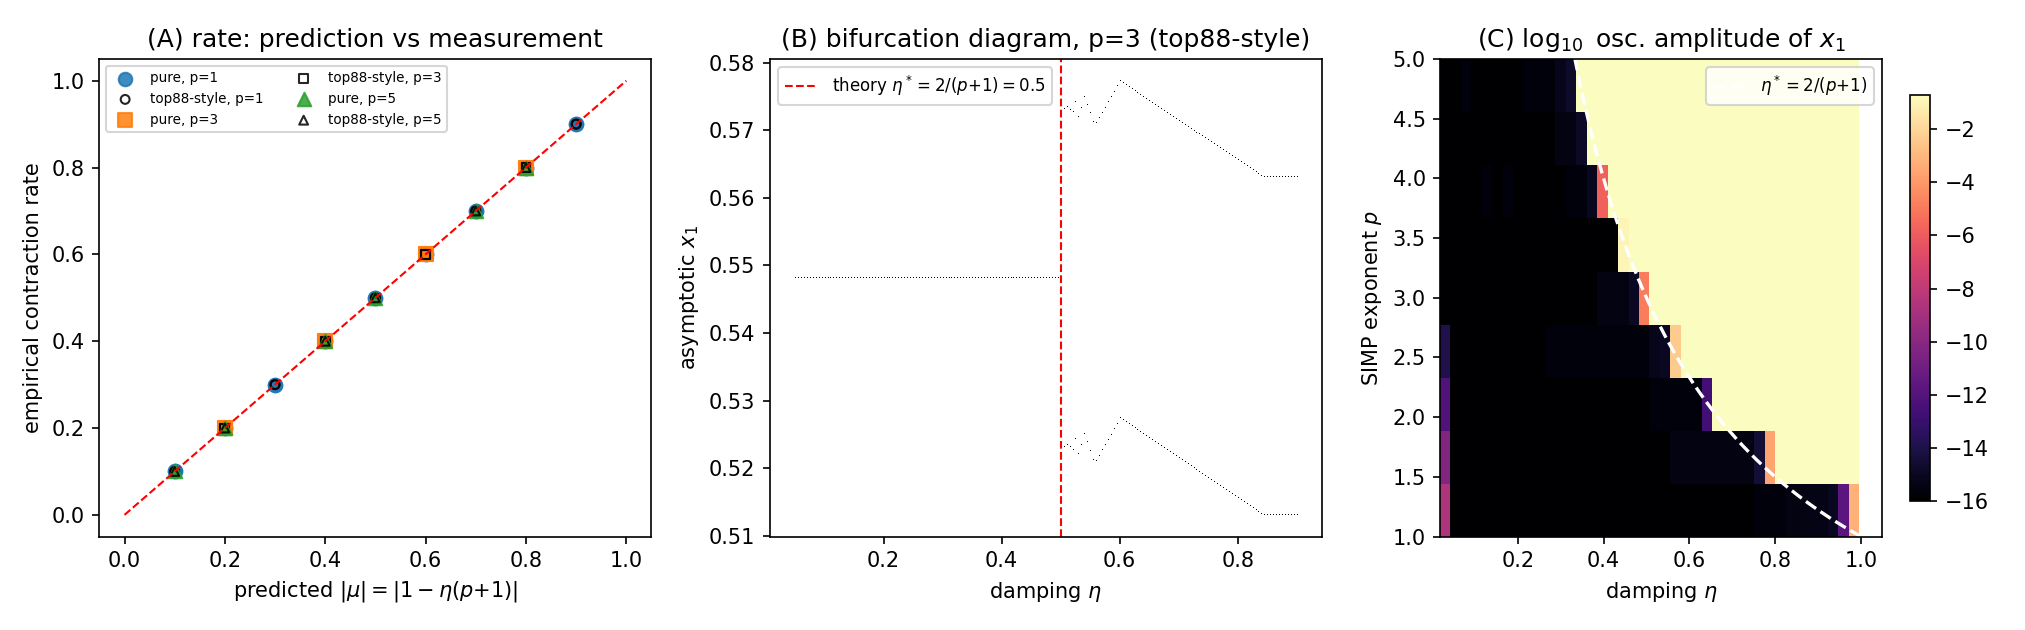
\includegraphics[width=\textwidth]{fig_cycle1.png}
\caption{Two-bar models (Section~\ref{sec:theory}). (A)~measured
contraction rates versus $|1-\eta(p{+}1)|$; (B)~bifurcation diagram at
$p=3$ splitting at $\eta=0.500$; (C)~oscillation amplitude in the
$(\eta,p)$ plane against the curve $\eta=2/(p{+}1)$; (D)~parallel-model
winner-take-all run. \todo{redraw as publication Fig.~1 with toy
schematics}}
\label{fig:toy}
\end{figure}

\begin{figure}[p]
\centering
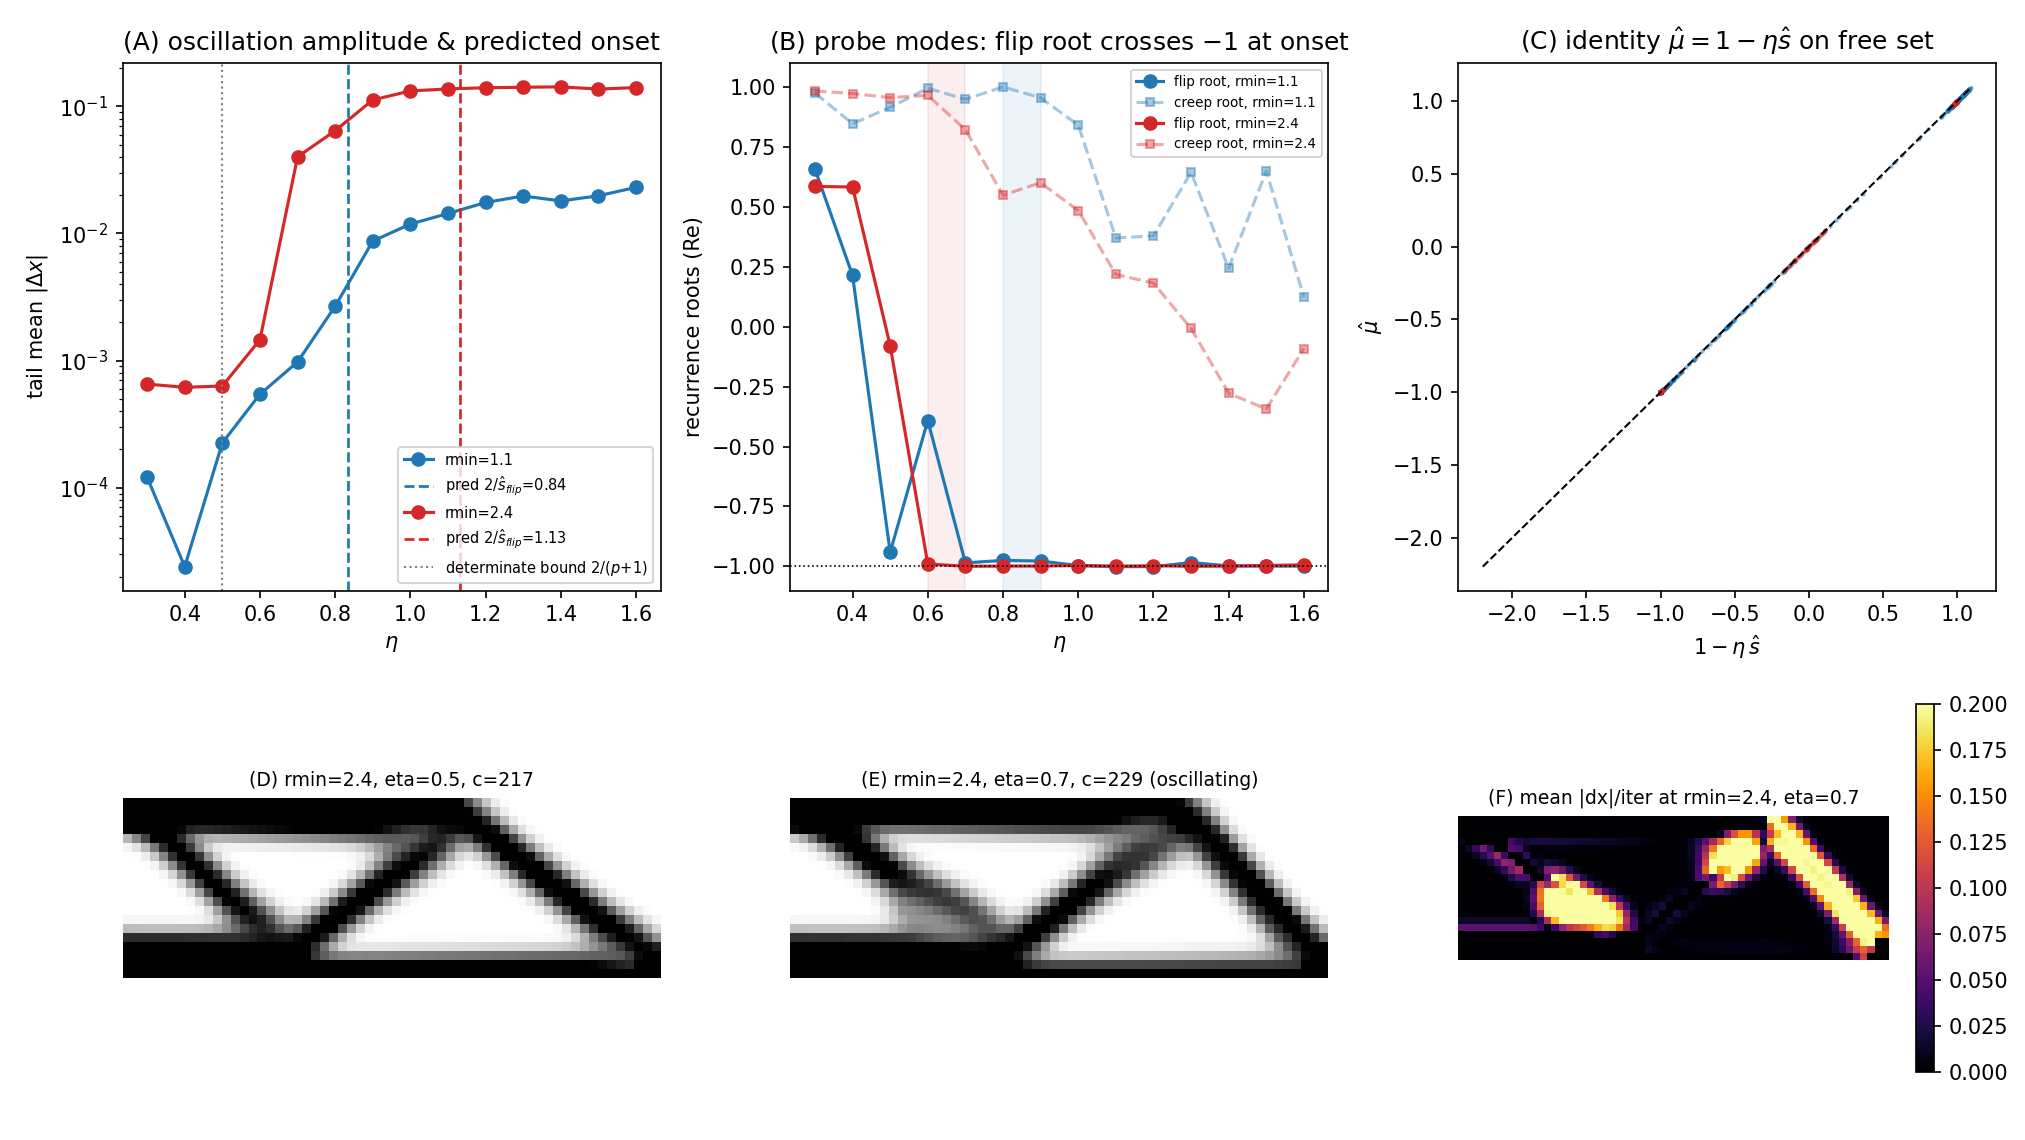
\includegraphics[width=\textwidth]{fig_cycle2.png}
\caption{The identity $\hat\mu=1-\eta\hat s$ across 28 instrumented runs
(three-decimal agreement), onset tags, and design snapshots
(Section~\ref{sec:identity}).}
\label{fig:identity}
\end{figure}

\begin{figure}[p]
\centering
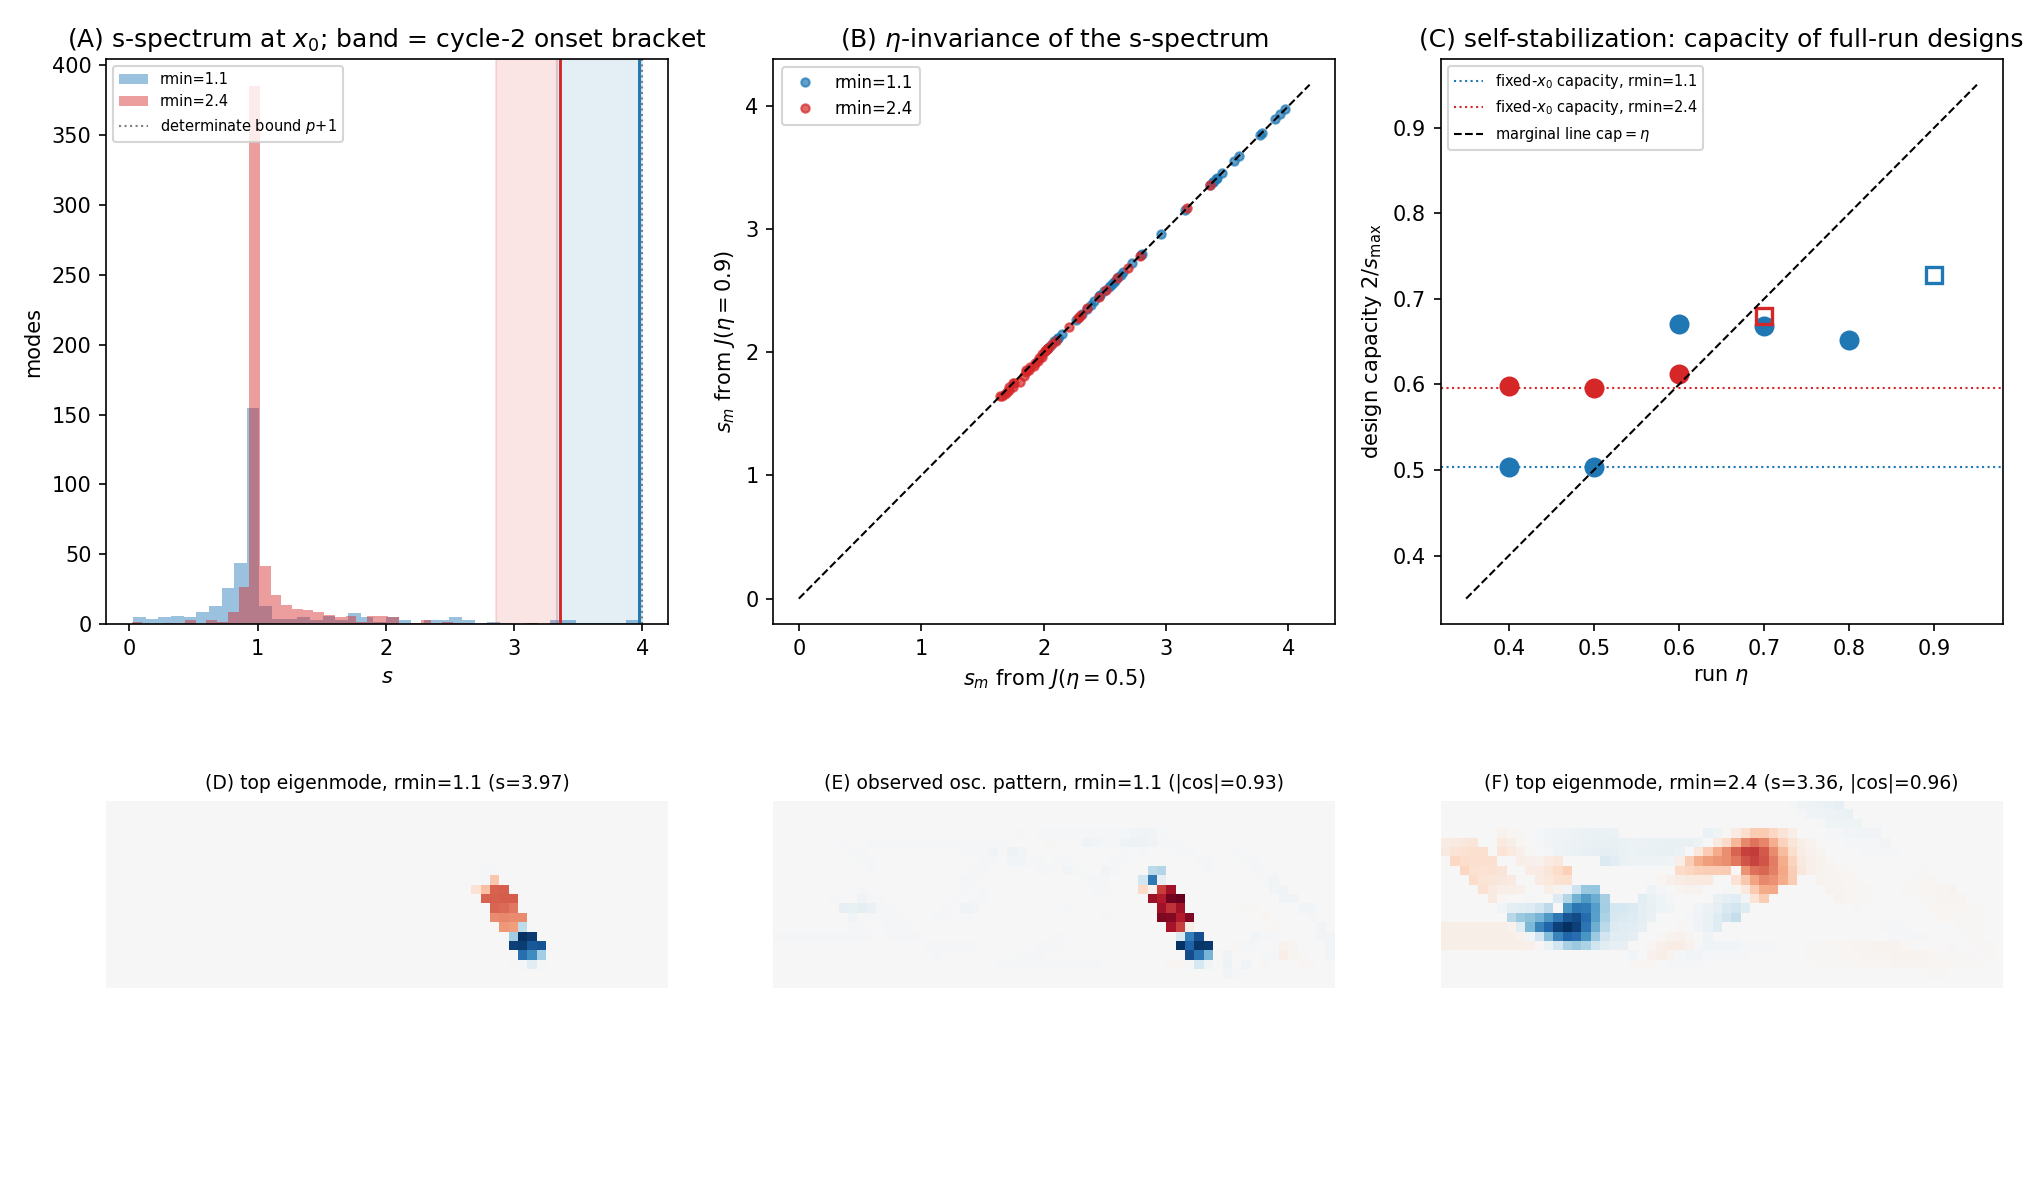
\includegraphics[width=\textwidth]{fig_cycle3.png}
\caption{Operator-level spectra (Section~\ref{sec:spectrum}):
$\eta$-invariant $s$-spectra, saturation of $\smax$ near $p{+}1$, and
leading eigenmodes versus observed oscillation patterns
($|\cos|\ge0.93$).}
\label{fig:spectrum}
\end{figure}

\begin{figure}[p]
\centering
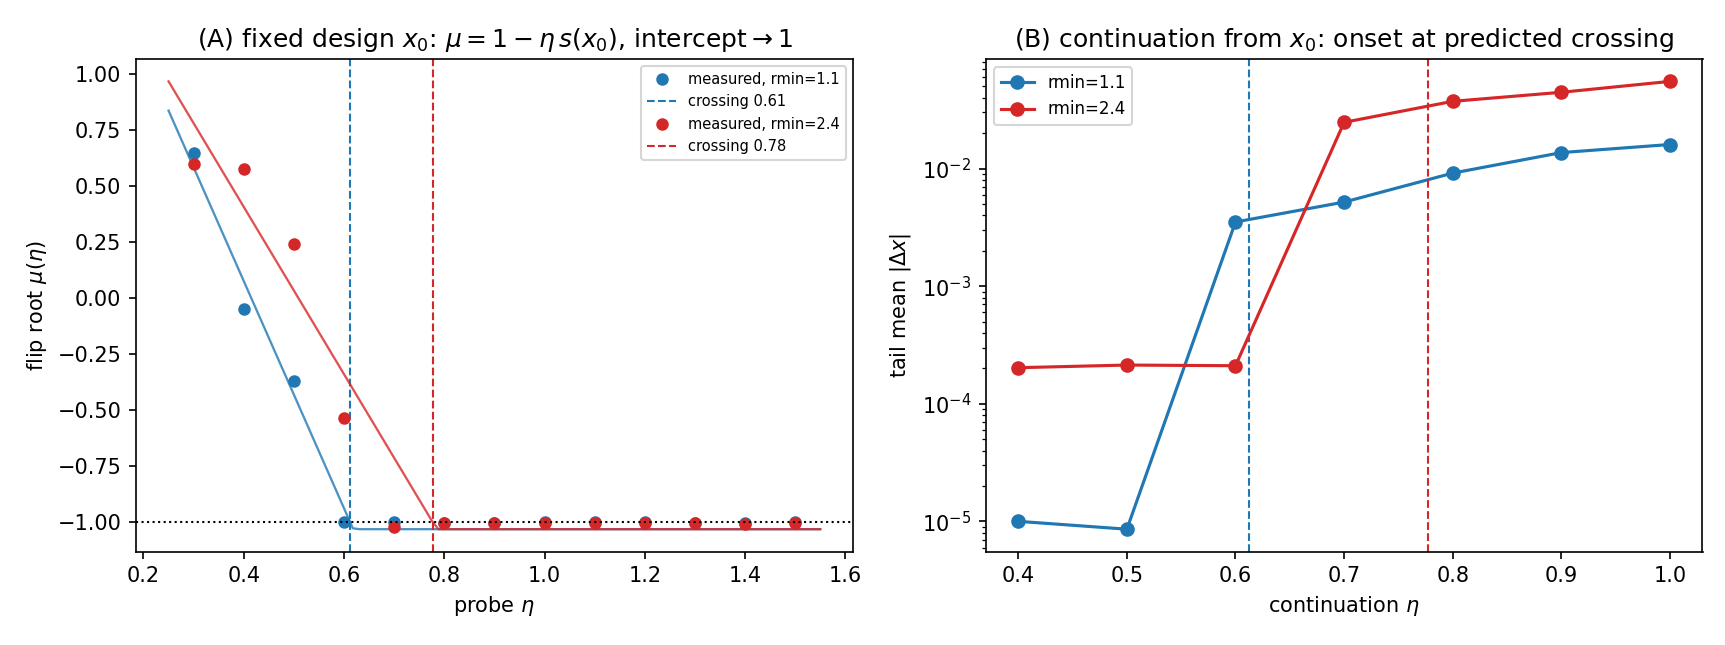
\includegraphics[width=\textwidth]{fig_cycle2c.png}
\caption{Fixed-design probes and capacity adaptation
(Section~\ref{sec:capacity}): flip roots versus $\eta$, and the
divergence between fixed-design thresholds and full-run onsets that the
capacity trajectory $2/\smax(\mathrm{design}(\eta))$ explains.}
\label{fig:capacity}
\end{figure}

\begin{figure}[p]
\centering
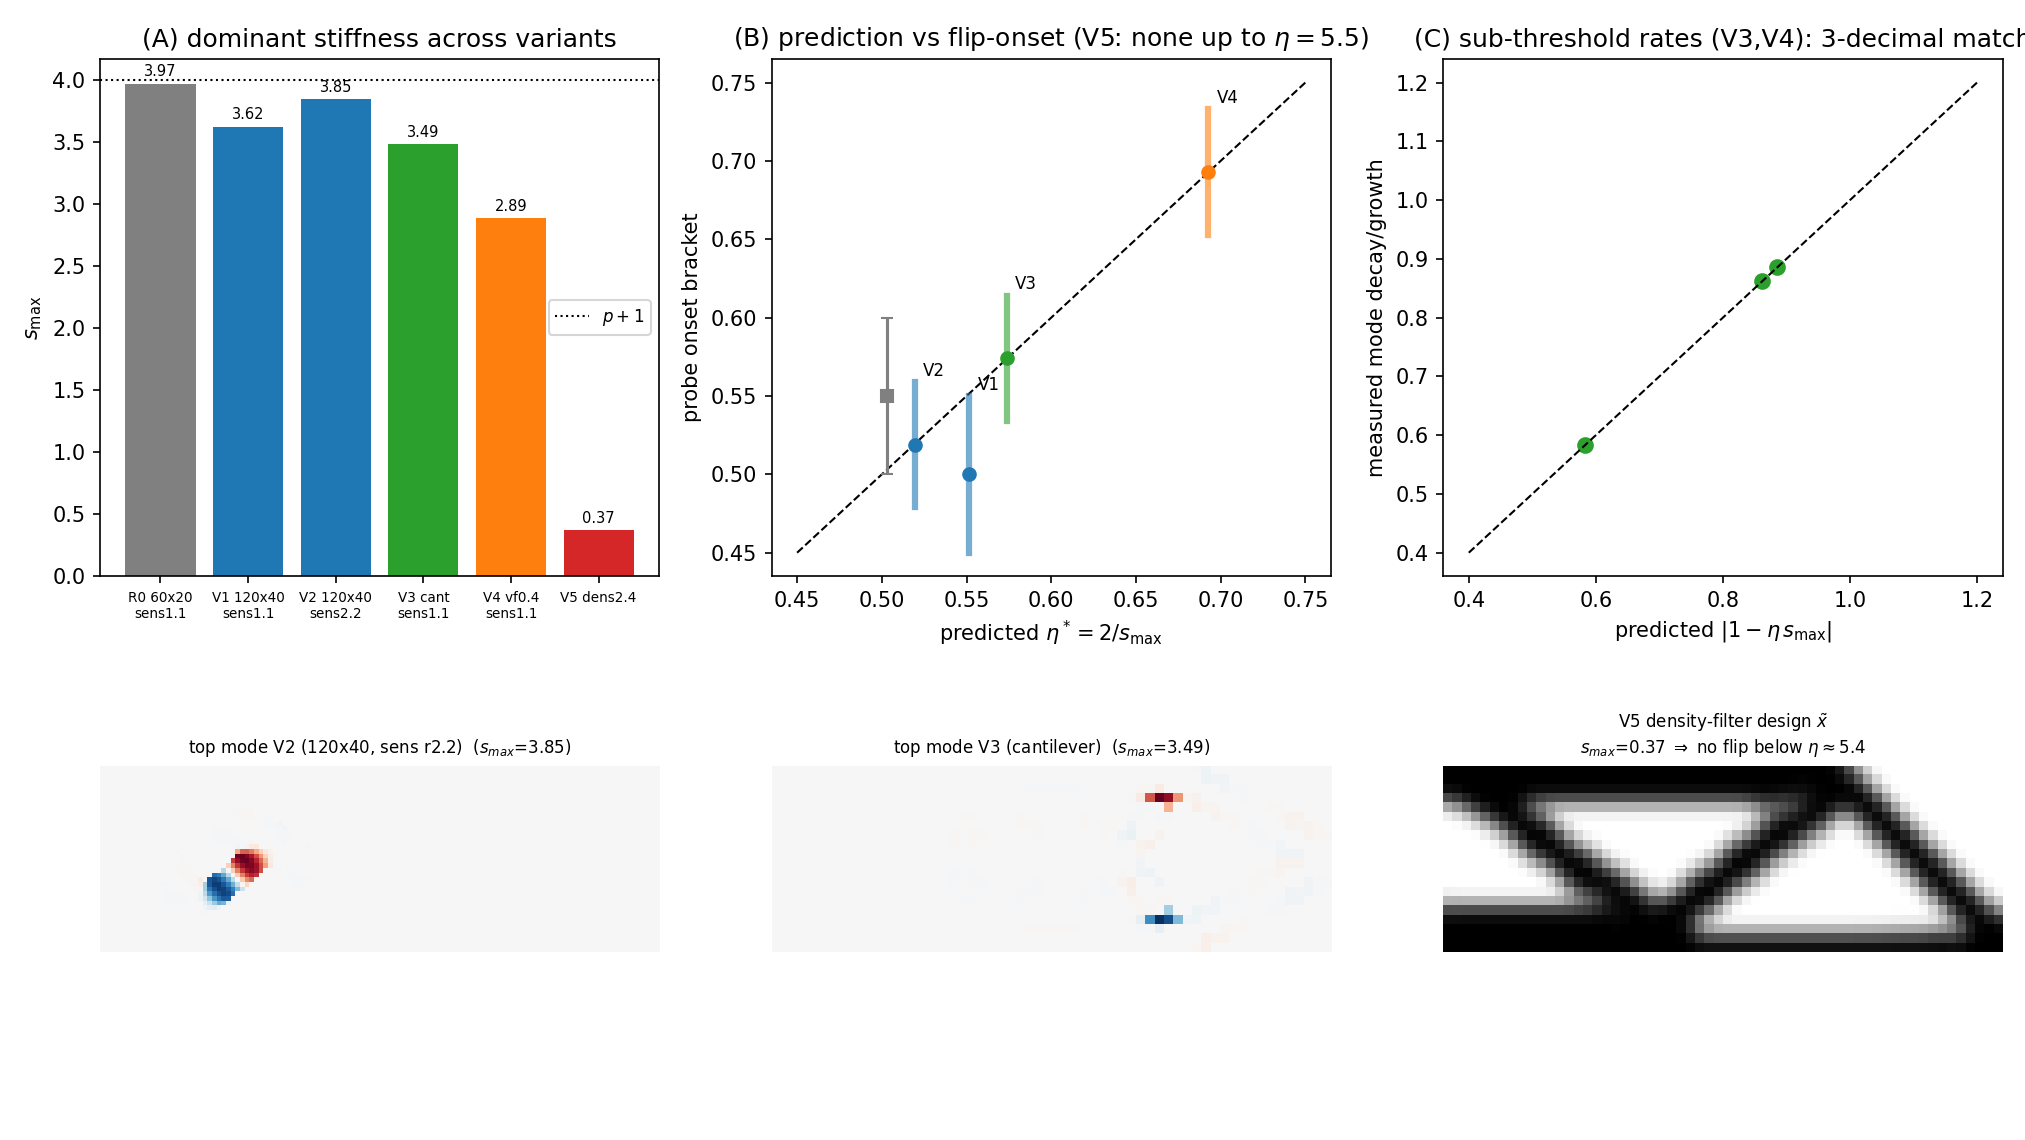
\includegraphics[width=\textwidth]{fig_cycle4.png}
\caption{Robustness sweep (Section~\ref{sec:robust}, Table~\ref{tab:robust}):
predicted $2/\smax$ versus behavioral onset brackets across mesh, boundary
conditions, volume fraction, and filter type; sub-threshold decay-rate
agreement to three decimals.}
\label{fig:robust}
\end{figure}

\begin{figure}[p]
\centering
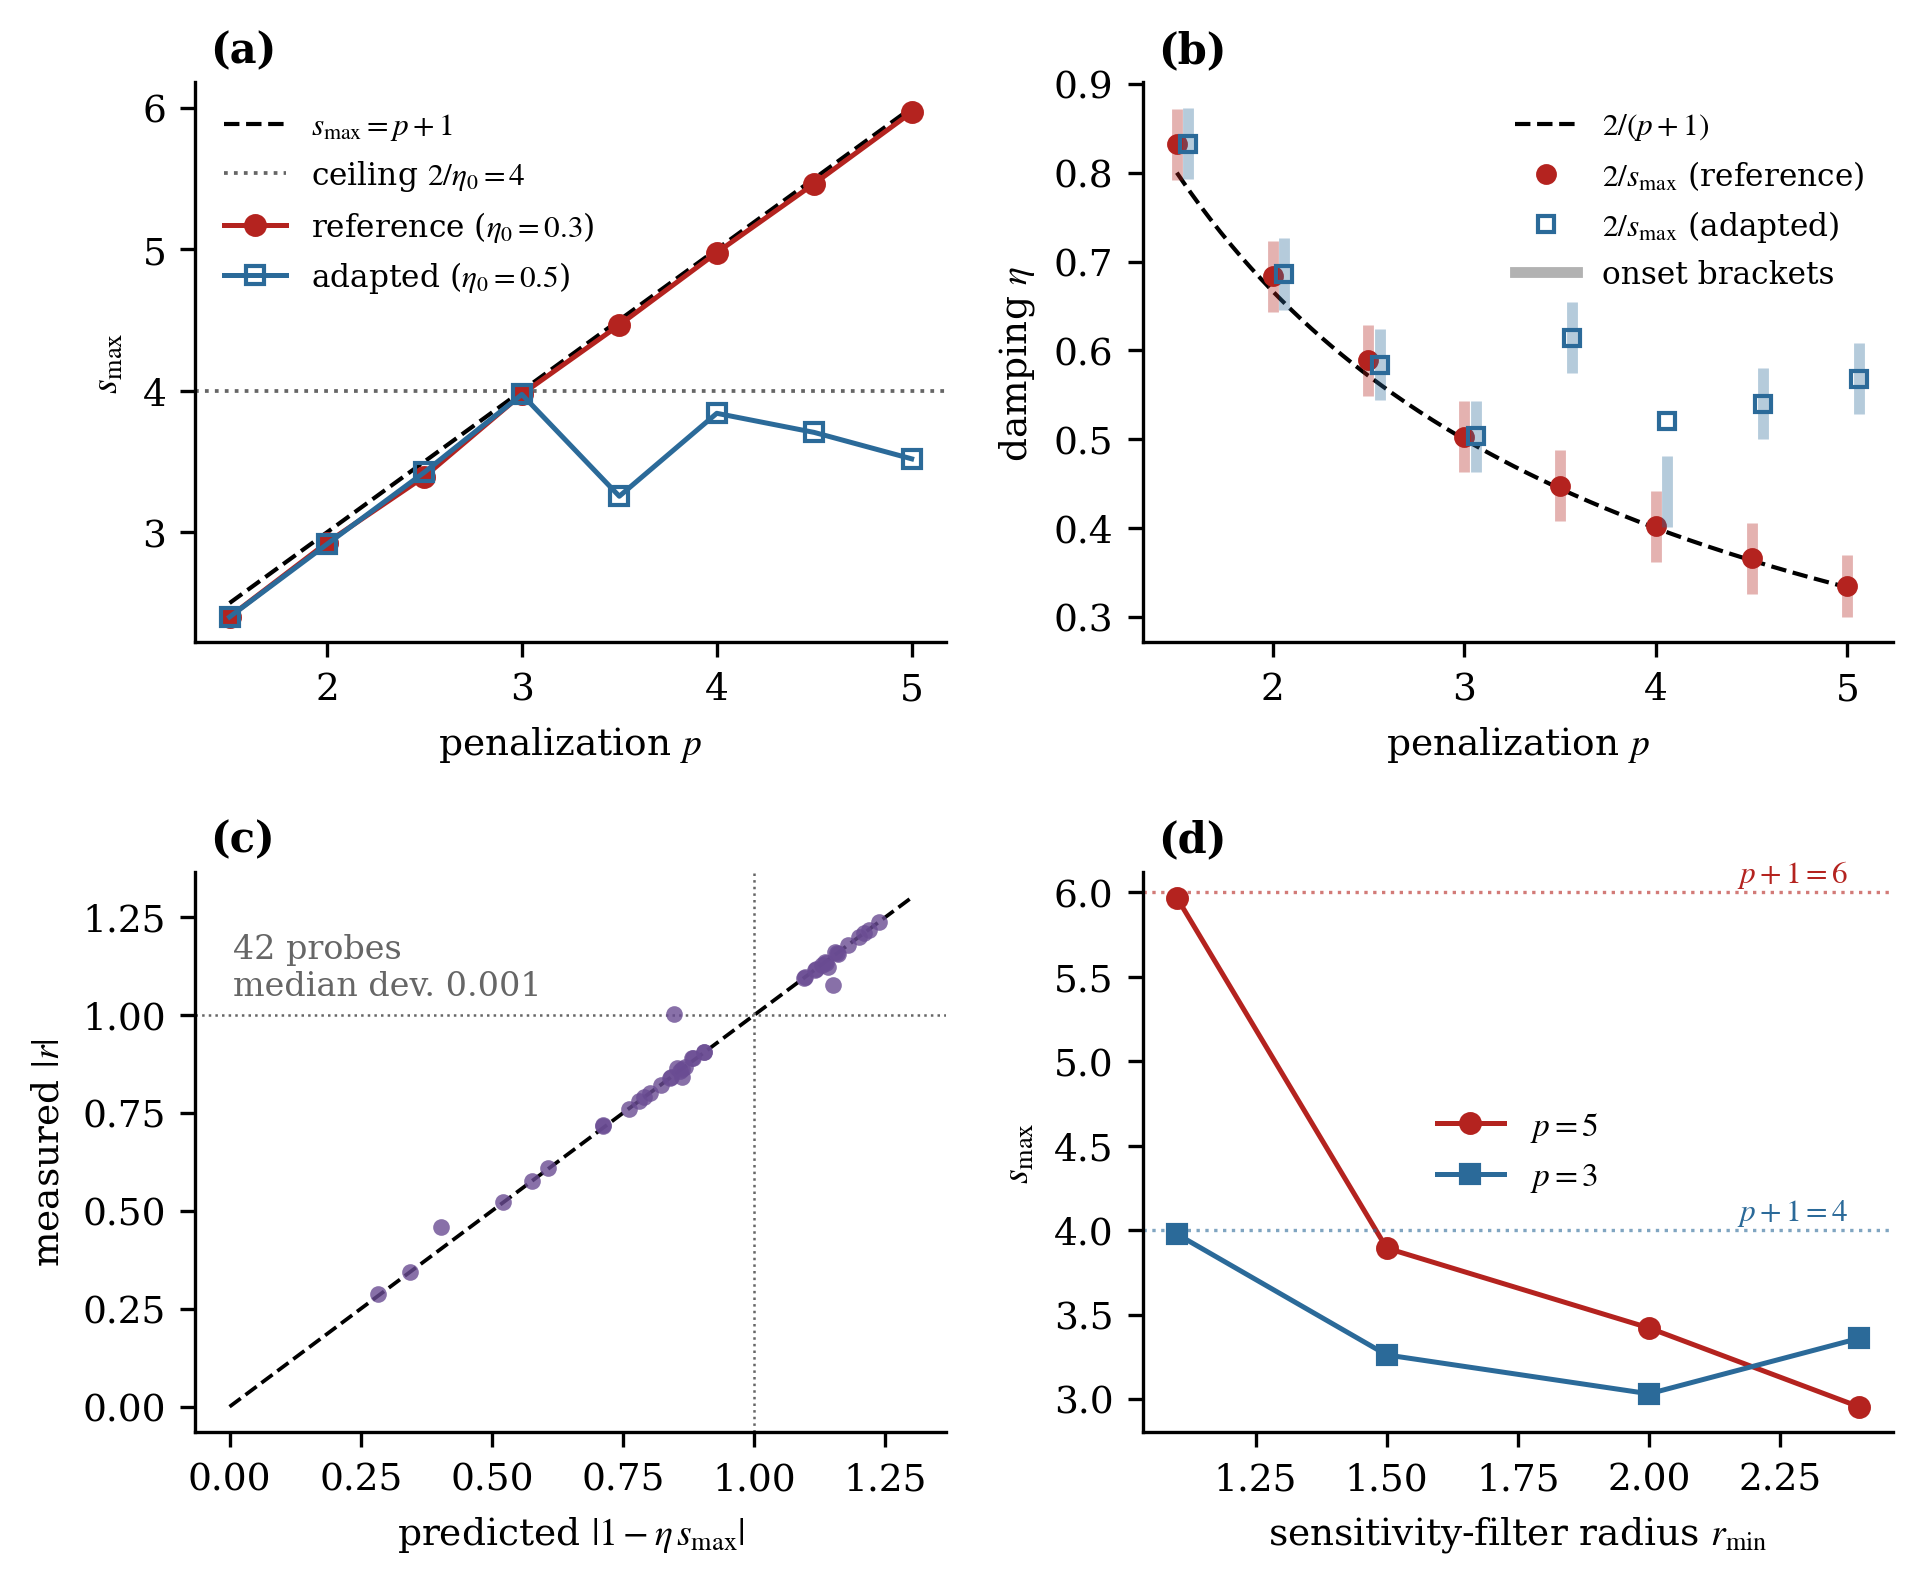
\includegraphics[width=0.92\textwidth]{fig_psweep_pub.png}
\caption{Penalization sweep (Section~\ref{sec:psweep}).
(a)~$\smax$ saturates at $p{+}1$ under the reference protocol (filled),
while the adapted protocol (open) pins below the capacity ceiling
$2/\eta_0=4$; the protocols separate exactly at $p=3$.
(b)~behavioral onset brackets follow each fixed point's own $2/\smax$
(at $p=5$: $0.335$ versus $0.568$).
(c)~rate law across both protocols: measured $|r|$ versus predicted
$|1-\eta\,\smax|$ for all flip-mode-active probes.
(d)~filter-radius detuning of $\smax$ at $p=3$ versus $p=5$
(reference protocol; cf.\ Table~\ref{tab:rmin}).}
\label{fig:psweep}
\end{figure}

\begin{figure}[p]
\centering
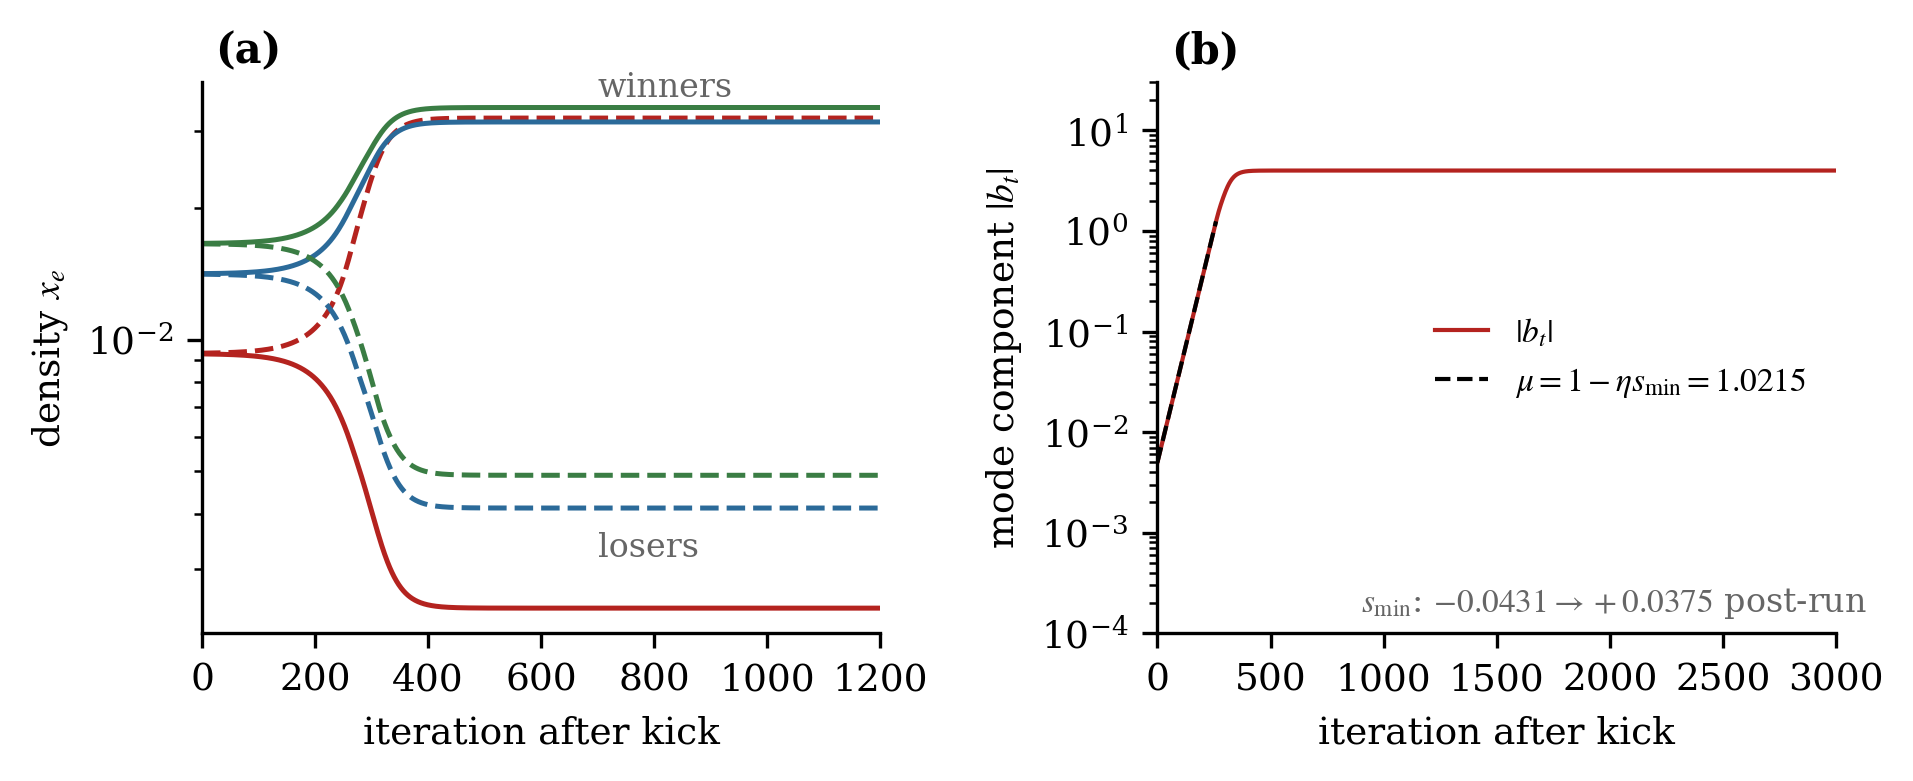
\includegraphics[width=0.92\textwidth]{fig_negbranch.png}
\caption{The negative branch on the cantilever (V3;
Section~\ref{sec:neg}). (a)~densities of the three strongest mirror pairs
(solid/dashed = pair partners): equal at the symmetric fixed point, split
by the kick into winners and losers, resettling within ${\sim}400$
iterations. (b)~mode component $|b_t|$: exponential growth at the
predicted rate $1-\eta\smin=1.0215$ (dashed), then a plateau at the new
asymmetric fixed point whose spectrum has shed the negative eigenvalue.}
\label{fig:negbranch}
\end{figure}

\begin{figure}[p]
\centering
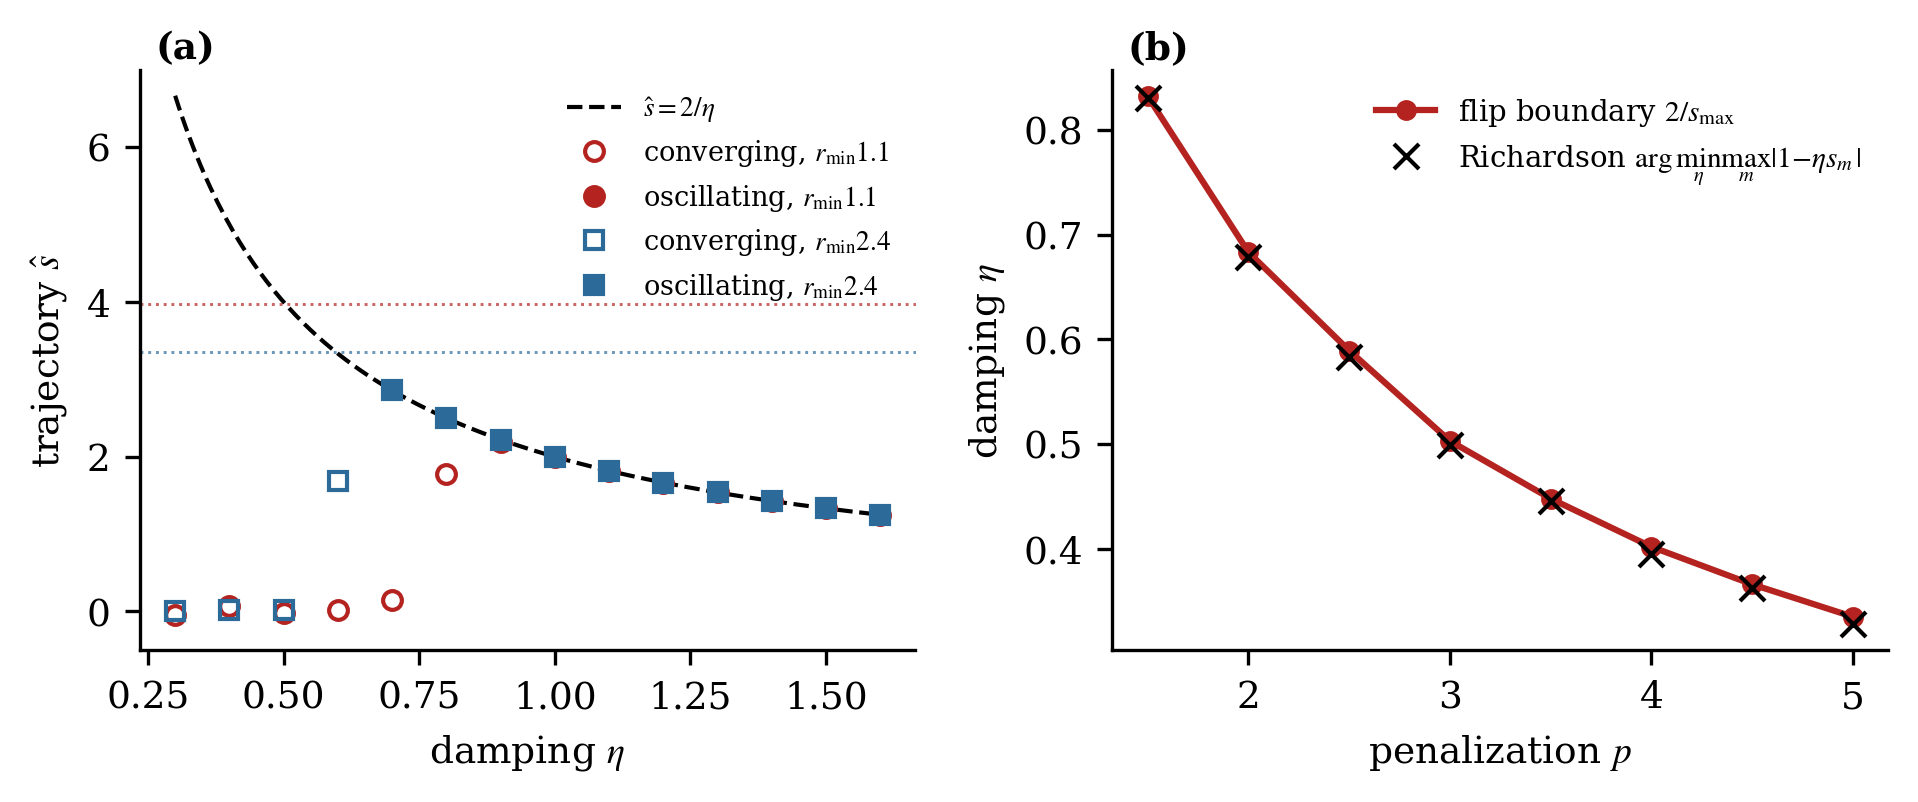
\includegraphics[width=0.92\textwidth]{fig_cycleA.png}
\caption{The two regimes of the trajectory estimator, and optimality of
the folklore damping (Sections~\ref{sec:identity}
and~\ref{sec:discussion}). (a)~trajectory $\hat s$ across the
$\eta$-sweep: converging runs (open) read the $s\approx0$ creep edge,
saturated runs (filled) lock onto $\hat s=2/\eta$ (dashed); dotted lines
mark the operator $\smax$ of the two $\eta{=}0.5$ designs.
(b)~the numerically computed min--max optimal damping
$\arg\min_\eta\max_m|1-\eta s_m|$ (crosses) coincides with the flip
boundary $2/\smax$ (line) across the penalization sweep.}
\label{fig:gate}
\end{figure}

\bibliographystyle{plainnat}
\bibliography{refs}

\end{document}
